

%############################################################################################
%############################################################################################
\section{Fixed Model-Driven MU-MIMO Evaluation}
\label{sec:model}
In order to understand how different environments and operational frequencies will effect the performance of a \ac{MU-MIMO} system, we first turn to modern statistical MIMO channel models \cite{liu2012cost}.
Since this statistical model requires tuning for different environments and frequencies, we compare the results using two published parametrizations  for 300~MHz \cite{zhu2013cost} and 5.8~GHz\cite{poutanen2011cost}. These results provide the theoretical motivation for over-the-air experiments to explore common application scenarios for UHF and 2.4/5.8~GHz WiFi.

\subsection{UHF vs. 2.4/5 GHz: Channel Models}
\label{sec:specDiff}

	Spectrum differences between 2.4/5~GHz WiFi and sub-gigahertz frequencies are essentially due to the different manifestations of Doppler effects given each band's wavelength.
	Doppler effects are a result of transmitter, receiver, and client movement with respect to a transmission's wavelength.  
	Because sub-gigahertz wavelengths are 2-4 times longer than 2.4/5~GHz, environmental variation will affect sub-gigahertz transmissions 2-4 times less (without considering multi-path effects).  

	Fig.~\ref{fig:doppler} shows the theoretical, freespace 50\% coherence time for various sub-gigahertz and 2.4/5~GHz frequencies \cite{rappaport1996wireless}.
	The 50\% coherence time is expected length of time that the channel characteristics will  vary at most 50\% given some velocity (effectively channel variation).

	The coherence time difference between 2.4/5~GHz WiFi and sub-gigahertz frequencies is between 1-2 \textit{orders of magnitude}.
	This channel characterization does not consider many real world effects such as multi-path or fading but provides a coarse characterization of the key differences in the two bands.

\begin{figure}[htbp!]
	\centering
  	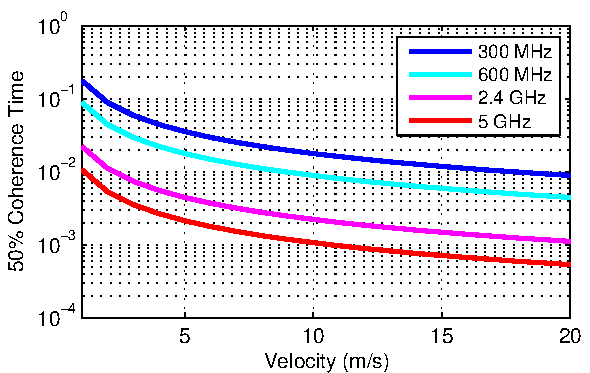
\includegraphics[width=0.7\linewidth]{figs/doppler}   
    	\caption{50\% coherence time for various sub-gigahertz and 2.4/5~GHz WiFi frequencies.}
	\label{fig:doppler}
\end{figure}

	For a more realistic characterization of the spectrum differences, we employ the COST 2100 MIMO channel model, a flexible channel model that is well suited for \ac{MU-MIMO} scenarios \cite{liu2012cost}.
	This channel model is tuned with parameters that are extracted from empirical measurements and thus does consider real-world channel effects such as fading,  multi-path, and \ac{NLoS} transmissions.
	Parametrized realizations of the COST 2100 model have been created for 300~MHz \cite{zhu2013cost} and 5~GHz \cite{poutanen2011cost} bands.
	Using these models, we generate 15,000 channel snapshots at a simulated rate of 100 snapshots per second to characterize the variation of channel state over time and the separability of individual users. 
	Specifically we explore the temporal correlation  and receiver separability  (shown in Fig.~\ref{fig:corr}) of the generated matrices.

\begin{figure}[ht]
	\centering
	\subfigure[Temporal correlation between channel snapshots from 0 to 10 seconds apart.  Higher time correlation allows for more robust MU-MIMO performance. $T_{0.9}$ is 50~ms and 4~s for 5 GHz and 300 MHz respectively.] {
	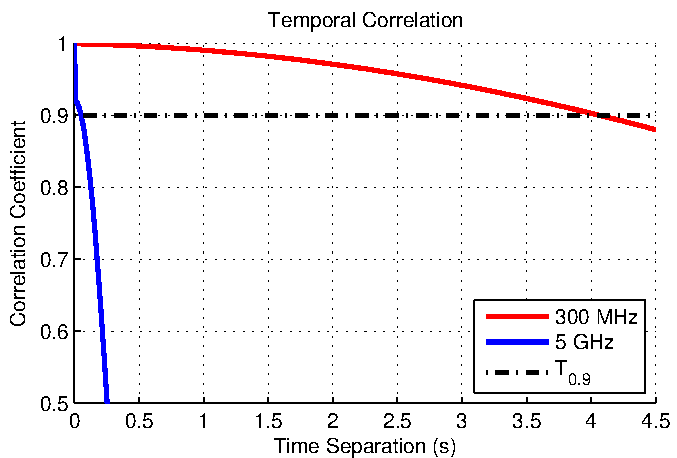
\includegraphics[width=0.48\linewidth]{figs/theo_tempDiff}
		\label{fig:theo_tempCorr}
	}
	\subfigure[CDF of model-generated Demmel condition number. Left is better for \ac{MU-MIMO}] {
		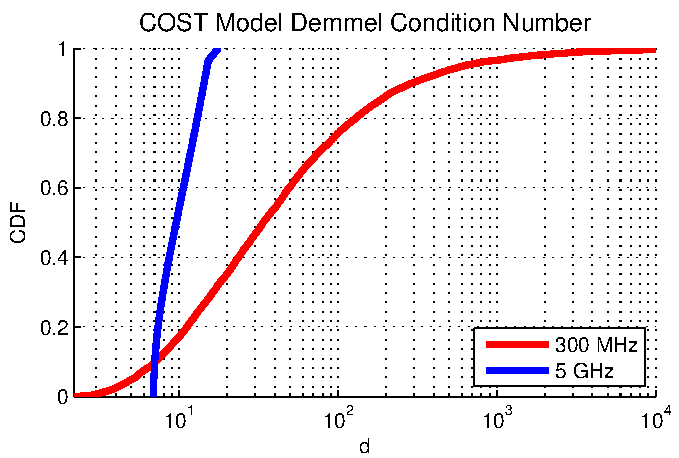
\includegraphics[width=0.48\linewidth]{figs/dcond_cdf}  
		\label{fig:spatCorr}
	}
  	\caption{Temporal correlation and channel condition of 300~MHz and 5~GHz 2x2 MU-MIMO channels generated by COST 2100 MIMO channel model. \label{fig:corr}} 
\end{figure}
 
	The correlation coefficient $\rho$ presented in Equation~\ref{eq_corr_coeff} is calculated for all combinations of transmit antenna, receive antenna, and starting time sample.
	We show the magnitude of the temporal correlation coefficient in Fig.~\ref{fig:theo_tempCorr} for our generated channels.  
	Lower temporal correlation results in less robust MU-MIMO transmissions because the measured channel state has a high probability of being stale.
	As seen in Fig.~\ref{fig:theo_tempCorr}, the temporal correlation of 5~GHz WiFi almost immediately drops to below 0.9 ($T_{0.9}$) a point when when re-sounding the channel is strongly suggested \cite{breit2009coherence}. 

According to the channel models, the approximate re-sounding time for 5~GHz is 50~ms and 300~MHz is approximately 4.5~s (almost two orders of magnitude longer). 
This result is similar to what we expect from Doppler effects of the different frequency bands (Fig.~\ref{fig:doppler}) and is similar to our indoor temporal characterization in \S~\ref{sec:indoor}.

\subsection{Demmel Condition Number}
\label{sec:demmel}

User separability refers to how well a multi-antenna transmitter can serve a set of users in parallel.  
The Demmel condition number is a modified matrix condition number that directly predicts the efficacy of an adaptive MIMO or MU-MIMO transmission for a particular channel realization \cite{zhong2011distribution}.

The Demmel condition number is computed using the eigenvalues $\lambda_k$ of $HH^{\dagger}$ as:
\begin{align}
d\triangleq\frac{\sum^{n}_{k=1}{\lambda_k}}{\lambda_{n}}
\label{eq:dcond}
\end{align}
where $\lambda_1 > \lambda_2 > \hdots > \lambda_n$.
This ratio represents how well a matrix can be inverted, a key component of many adaptive MU-MIMO techniques such as Zero-Forcing Beamforming \cite{goldsmith2006zf} and MMSE \cite{tse2005fundamentals}.
Specifically, the higher the condition number, the more numerically unstable the inverse and thus the more inter-user interference during MU-MIMO transmissions reducing received SINR.  
The condition number ranges from 1 to infinity for well to ill-conditioned matrices, respectively.  

This method of calculating the condition number is less forgiving than the traditional singular value ratio. 
The singular values of $H$ are the square root of the eigenvalues of $HH^{\dagger}$.
Thus, instead of $\sigma_k/\sigma_n$, the Demmel condition number is equivalent to $\sum{\sigma^2}/\sigma_n^2$ meaning that channel matrices with low singular values (resulting in inaccurate inversion) are even further ``penalized.``
This modification to the condition number better predicts MU-MIMO performance, in fact, it is consistent and accurate enough to be used for determining parameters such as supported modulation rate and user selection \cite{zhong2011distribution}.


The COST channel models show a significant difference between the 5~GHz WiFi and UHF bands.  
The CDF shown in Fig.~\ref{fig:spatCorr} depicts how almost all of the generated 5~GHz channel matrices have a Demmel condition number less than 10 while UHF's channel condition varies far more and is significantly worse.
This results in an increased ability for a \ac{MU-MIMO} transmitter to invert the channel matrix and send orthogonal streams to each intended user. 


Thus, existing MIMO channel models show that while the UHF channel is more temporally stable over time, its ill-conditioned channel matrices can result in lower served SINR due to inter-user interference. 
However, the available parametrizations of the COST model are for indoor 5~GHz  and outdoor UHF scenarios.  
%We show in \S~\ref{sec:expDrivenEval} how restricting these bands to these transmission environments does not tell the full story.

\section{Fixed Indoor MU-MIMO Channel Characterization}
\label{sec:mumimo_channels} 

%############################################################################################
%############################################################################################
%\subsection{Experiment-Driven Fixed Wireless Evaluation}
%\label{sec:expDrivenEval}
The models analyzed in Section~\ref{sec:model} are parametrized for particular environments, frequency bands, and topologies. While they suggest that the performance of \ac{MU-MIMO} beamforming in UHF bands may be advantageous, it it difficult to directly predict or simulate UHF performance using these models as they were not validated for application scenarios such as indoor or urban outdoor, nor the UHF frequency band.

In order to address uncertainty in these models for our target application (indoor and outdoor \ac{WLAN}), we perform a set of  experiments utilizing our custom \ac{SDR} radio platform that allows us to measure the performance of a \ac{MU-MIMO} transmission over a diverse set of carrier frequencies and characterize the wireless \ac{MU-MIMO} channel for important temporal and spatial correlation properties.

We perform over-the-air beam-forming transmissions in a densely packed, challenging office scenario with multiple subscriber nodes and demonstrate not only the ability to simultaneously beamform to distinct users in relatively close proximity, but also the relative improvement that shifting to UHF frequencies provides.

Finally, we perform two sets of experiments with a customized MAC and PHY designed to gather dense, wideband, over-the-air channel estimates in realistic indoor and outdoor \ac{WLAN} scenarios with multiple subscriber nodes. Using this data, we then demonstrate that the spatial correlation for outdoor users remains similar to that of 2.4~GHz WiFi, thus incurring no beamforming ``penalty'' for utilizing a frequency band with superior propagation and temporal correlation.

\subsection{Indoor MU-MIMO Transmissions}
\label{sec_static_indoor_exp}

\label{sec:indoor}
\textbf{Experimental Setup.}
First, we evaluate the performance of UHF \ac{MU-MIMO} in an indoor \ac{NLoS}  office environment.
Experiments were conducted during the work day with people walking through the halls in the environment depicted in Fig.~\ref{fig:indoorExp}.


\begin{figure*}[t!]
	\centering
  	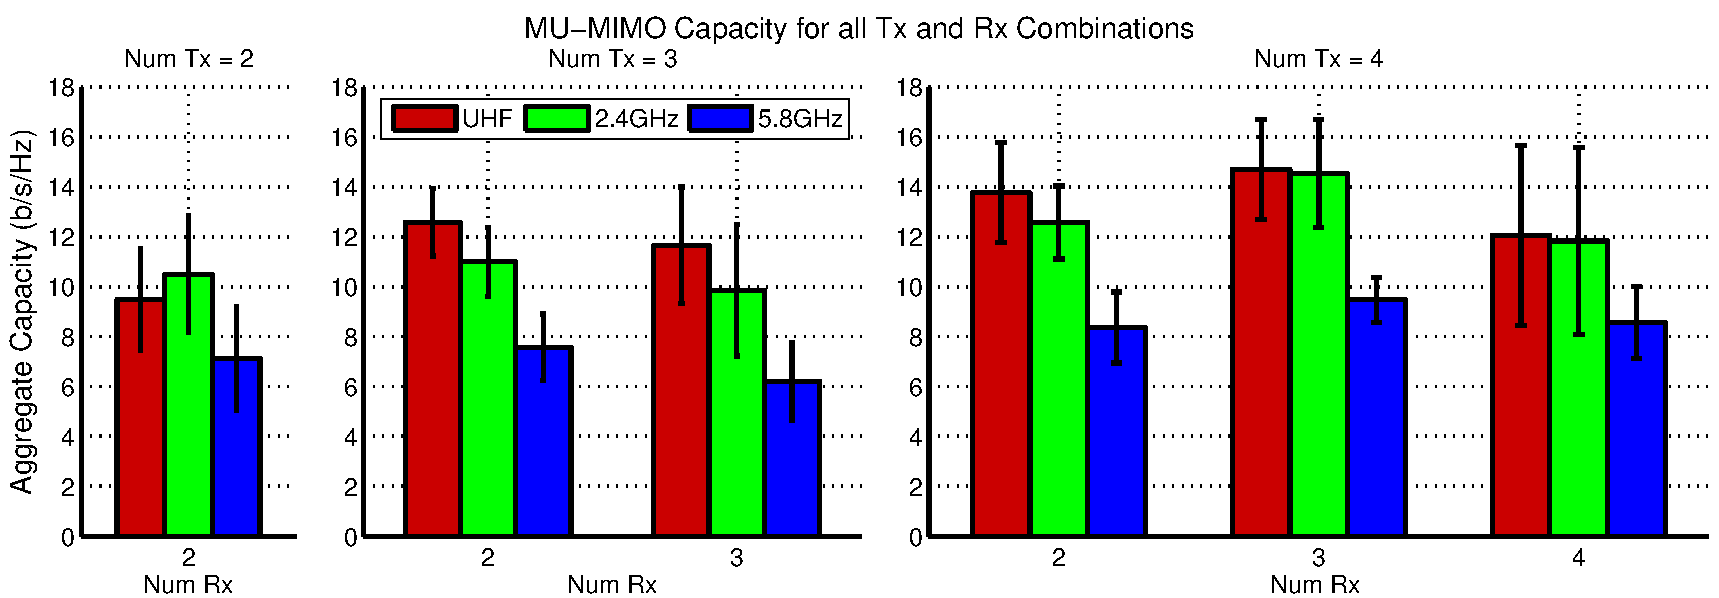
\includegraphics[width=1\linewidth]{figs/indoor_wl_all}   
    	\caption{Indoor fixed MU-MIMO achievable rate.\label{fig:indoor_cap_all}}
\end{figure*}


\begin{figure}[th]
\vspace{-5mm}
	\centering
  	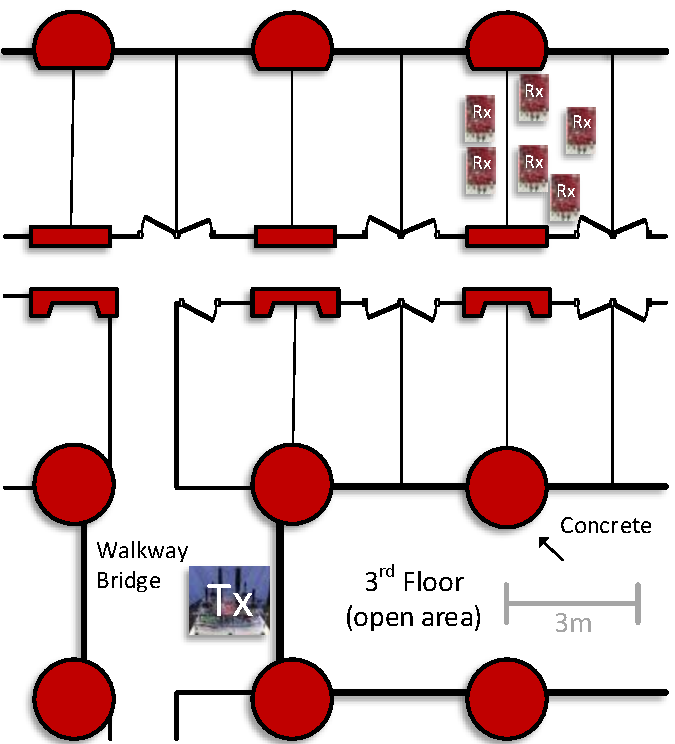
\includegraphics[width=0.7\linewidth]{figs/indoorExp}   
    	\caption{Indoor fixed WURC-based experimental test setup.
	\label{fig:indoorExp}}
\end{figure}


The \hspace{0.01pt} transmitting \hspace{0.01pt} array\hspace{0.01pt}  was \hspace{0.01pt}  placed \hspace{0.01pt} on \hspace{0.01pt} a \hspace{0.01pt} third \hspace{0.01pt} floor \hspace{0.01pt} walkway bridge and 6 separate receivers in two adjacent offices within the adjoining hallway.
Note that the to-scale depiction in Fig.~\ref{fig:indoorExp} shows the relative co-location of all receiving nodes with respect to the distance from the transmitter to simulate a densely packed office environment.
This represents a realistic, challenging case for indoor stationary MU-MIMO transmissions due to the co-located receivers.

To encompass a wide range of user grouping conditions, every possible combination of transmit and receive antennas are considered. Sixty transmissions are performed for each topology. The center frequencies for each frequency band (\textit{i.e.} channel) were chosen so that transmissions did not encounter interference from other equipment. Specifically, the UHF channel was first directly scanned for existing DTV or microphone transmissions and an experimental license was obtained to operate equipment on that channel. The channels selected for 2.4 and 5.8 GHz are not currently supported by the regulatory domain where these experiments were performed, thus ensuring minimal ISM-band interference.
	Using the measurement technique specified in Section~\ref{sec_static_miso_chan_est}, every possible topology's MU-MIMO capacity is measured for each frequency band and shown in Fig.~\ref{fig:indoor_cap_all}.



\begin{figure}[th]
		\centering  
	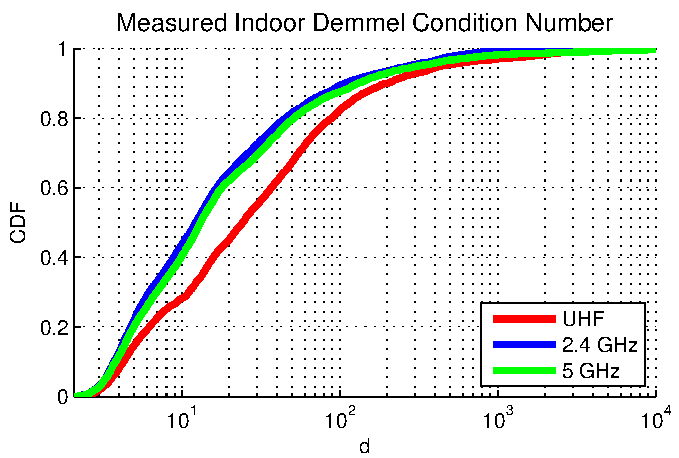
\includegraphics[width=0.7\linewidth]{figs/meas_indoor_dcond} 
    	\caption{Demmel condition number measured for the indoor environment. Left is better for \ac{MU-MIMO}.
	\label{fig:indoor_demmel}}
\end{figure}


      
\subsubsection{Fixed Wireless Measured Achievable Sum-Rate Capacity.}

Based on the channel models and accompanying analysis presented in Section~\ref{sec:specDiff}, we expect that the increased spatial correlation of UHF channels will not \  allow \ for \ MU-MIMO \ transmissions\ to \ accurately separate nearby users.
However, we find that UHF \ac{MU-MIMO} transmissions can actually achieve a sum capacity similar to that of 2.4~GHz WiFi transmissions (always between 1-2~b/s/Hz above of below the 2.4~GHz band).

In fact, we find that majority of the intuition and channel models surrounding UHF MU-MIMO are not specific to the frequency band itself but rather generalized characteristics of MU-MIMO transmissions.
For example, the available MU-MIMO channel models characterize \textit{indoor} WiFi and \textit{outdoor} UHF channel environments where, regardless of frequency band, we expect increased difficulty in user separability in outdoor environments.  
Note the channel condition of the different transmission bands in the NLOS environment in Figure~\ref{fig:indoor_demmel} are similar in contrast to Fig.~\ref{fig:spatCorr}.  
Even though the wavelength of UHF is longer resulting in better propagation through materials, the UHF-band transmission still experiences enough multi-path to successfully beamform to multiple users in parallel.



Additionally, the results shown in Figure~\ref{fig:indoor_cap_all} show a known trend of achievable capacity for MU-MIMO transmissions where the MU-MIMO gain plateaus as the available \ac{DoF}\footnote{\ac{DoF} here refers to how many more transmit antennas there are than receive antennas in a MIMO transmission.} are reached.
The consistently worse performance of 5.8~GHz is explained by the high attenuation experienced by that frequency band in \ac{NLoS} conditions combined with its sensitivity to environmental variation.    

Note that UHF MU-MIMO consistently outperforms 2.4~GHz transmissions except for in the 2x2 transmission scenario.  
Because the sum transmit power emanating from the array is held constant regardless of the number of transmit antennas in use, the performance differential is solely a result of channel state, specifically it is an indicator of temporal channel correlation due to the WARPLab measurement platform.


	As discussed in Section~\ref{sec_warplab_timing}, the latency in the WARPLab platform is due to the rate at which the host PC can download and upload samples to each of the WARP boards over Ethernet. 
	In our system, we benchmark a read/write rate of approximately 2.5~ms per buffer and the closed loop beamforming method employed requires between  10 to 20~ms to complete depending on the number of transmit and receive antennas (the difference between a 2x2 and 4x4 transmission scenario).


\subsection{Fixed Wireless Measured Temporal Correlation.}
\label{sec_fixed_temporal}

To gain additional insight into the measured capacity results and to infer real world performance from 
our MU-MIMO transmissions, we also consider the channel correlation measured during each experiment.

For each topology, we consider each of the 60 MU-MIMO transmissions and their channel matrices.
We calculate channel correlation between varying times during the experiment to measure the rate of change of the channel information with respect to time.  
These calculations are an average over all topologies (all combinations of transmit and receive antennas).


\begin{figure}[th]
	\centering
 	 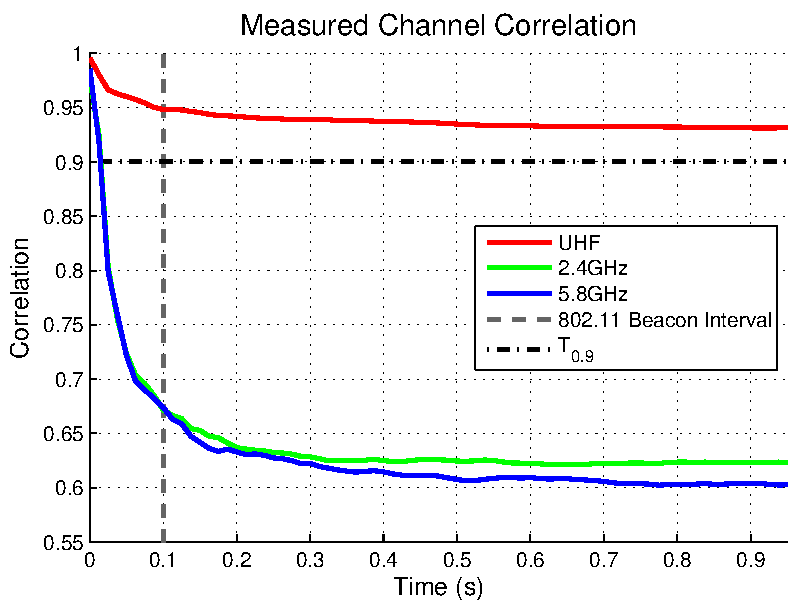
\includegraphics[width=0.7\linewidth]{figs/measCorrWl}   
   	 \caption{Measured Temporal Channel Correlation, depicting Beacon Interval, and $T_{0.9}$.  WARPLab latency is 10-20~ms depending number of transmit and receive antennas.
	\label{fig:meas_corr}}
\end{figure}


Fig.~\ref{fig:meas_corr} shows how the channels decorrelate over the course of one measured second in time.
This is effectively an indicator of how long a transmitter has after measuring the channel matrix and before actually transmitting parallel streams using that measurement.  
A coherence time of $T_{0.9}$ represents when the probability of the channel being too stale to successfully beamform over is high.

First, note that the WARPLab latency range of 10 to 20~ms is approximately $T_{0.9}$ for the 
the two WiFi frequency bands.
This indicates why only the 2x2 transmission scenario has the 2.4~GHz transmitter outperform UHF MU-MIMO; the latency between the sounding and transmission phase was the lowest and just at the $T_{0.9}$ limit.

While the 2.4/5~GHz frequencies both drop significantly within 100~ms, UHF remains above the $T_{0.9}$  threshold for the maximum one measured second difference between channel matrices.  
While these correlation values are not asymptotic and will eventually degrade, the performance of 2.4 and 5.8~GHz is sufficently low for stationary devices \cite{breit2009coherence}. 

The 802.11 infrastructure \ac{BSS} beacon rate\footnote{The IEEE Std 802.11-2012 Target Beacon Transmission Time (TBTT) is configured in ``Time Units'' defined as 1 TU = 1024 $\mu s$, and is often set to 100~TU.} (102.4~ms \cite{std11_2012}) is greater than the interval that 2.4/5~GHz MU-MIMO channels decorrelate.  
However, the stability of the UHF channel implies that a UHF MU-MIMO system could use periodic protocol packets for exchanging channel state information. 

Finally, the channel correlation result shown in Fig.~\ref{fig:meas_corr} effectively scales the MU-MIMO achievable rate shown in Fig.~\ref{fig:indoorExp}.
The rate at which the 2.4/5~GHz channel decorrelates necessitates channel sounding on a per packet basis adding considerable overhead to MU-MIMO transmissions. 
However, the temporal stability of the UHF MU-MIMO channel allows a transmitter to significantly reduce this overhead intensive sounding process and thus significantly increase the potential MU-MIMO gains. 

%############################################################################################
%############################################################################################

\begin{figure}[p]
	\centering
	\subfigure[Experimental setup for outdoor channel sounding.] {
	\centering
	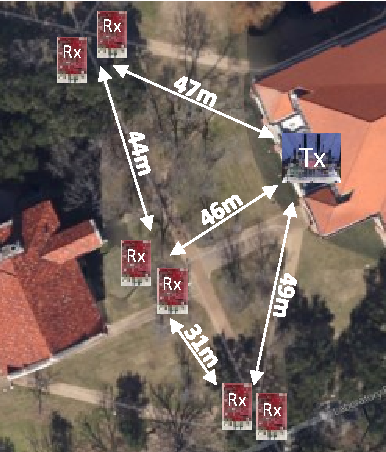
\includegraphics[width=0.48\linewidth]{figs/meas/outdoorExp}
		\label{fig_fix_outdoor_diagram}
	}
	\subfigure[Example of outdoor STA with dual antennas.] {
		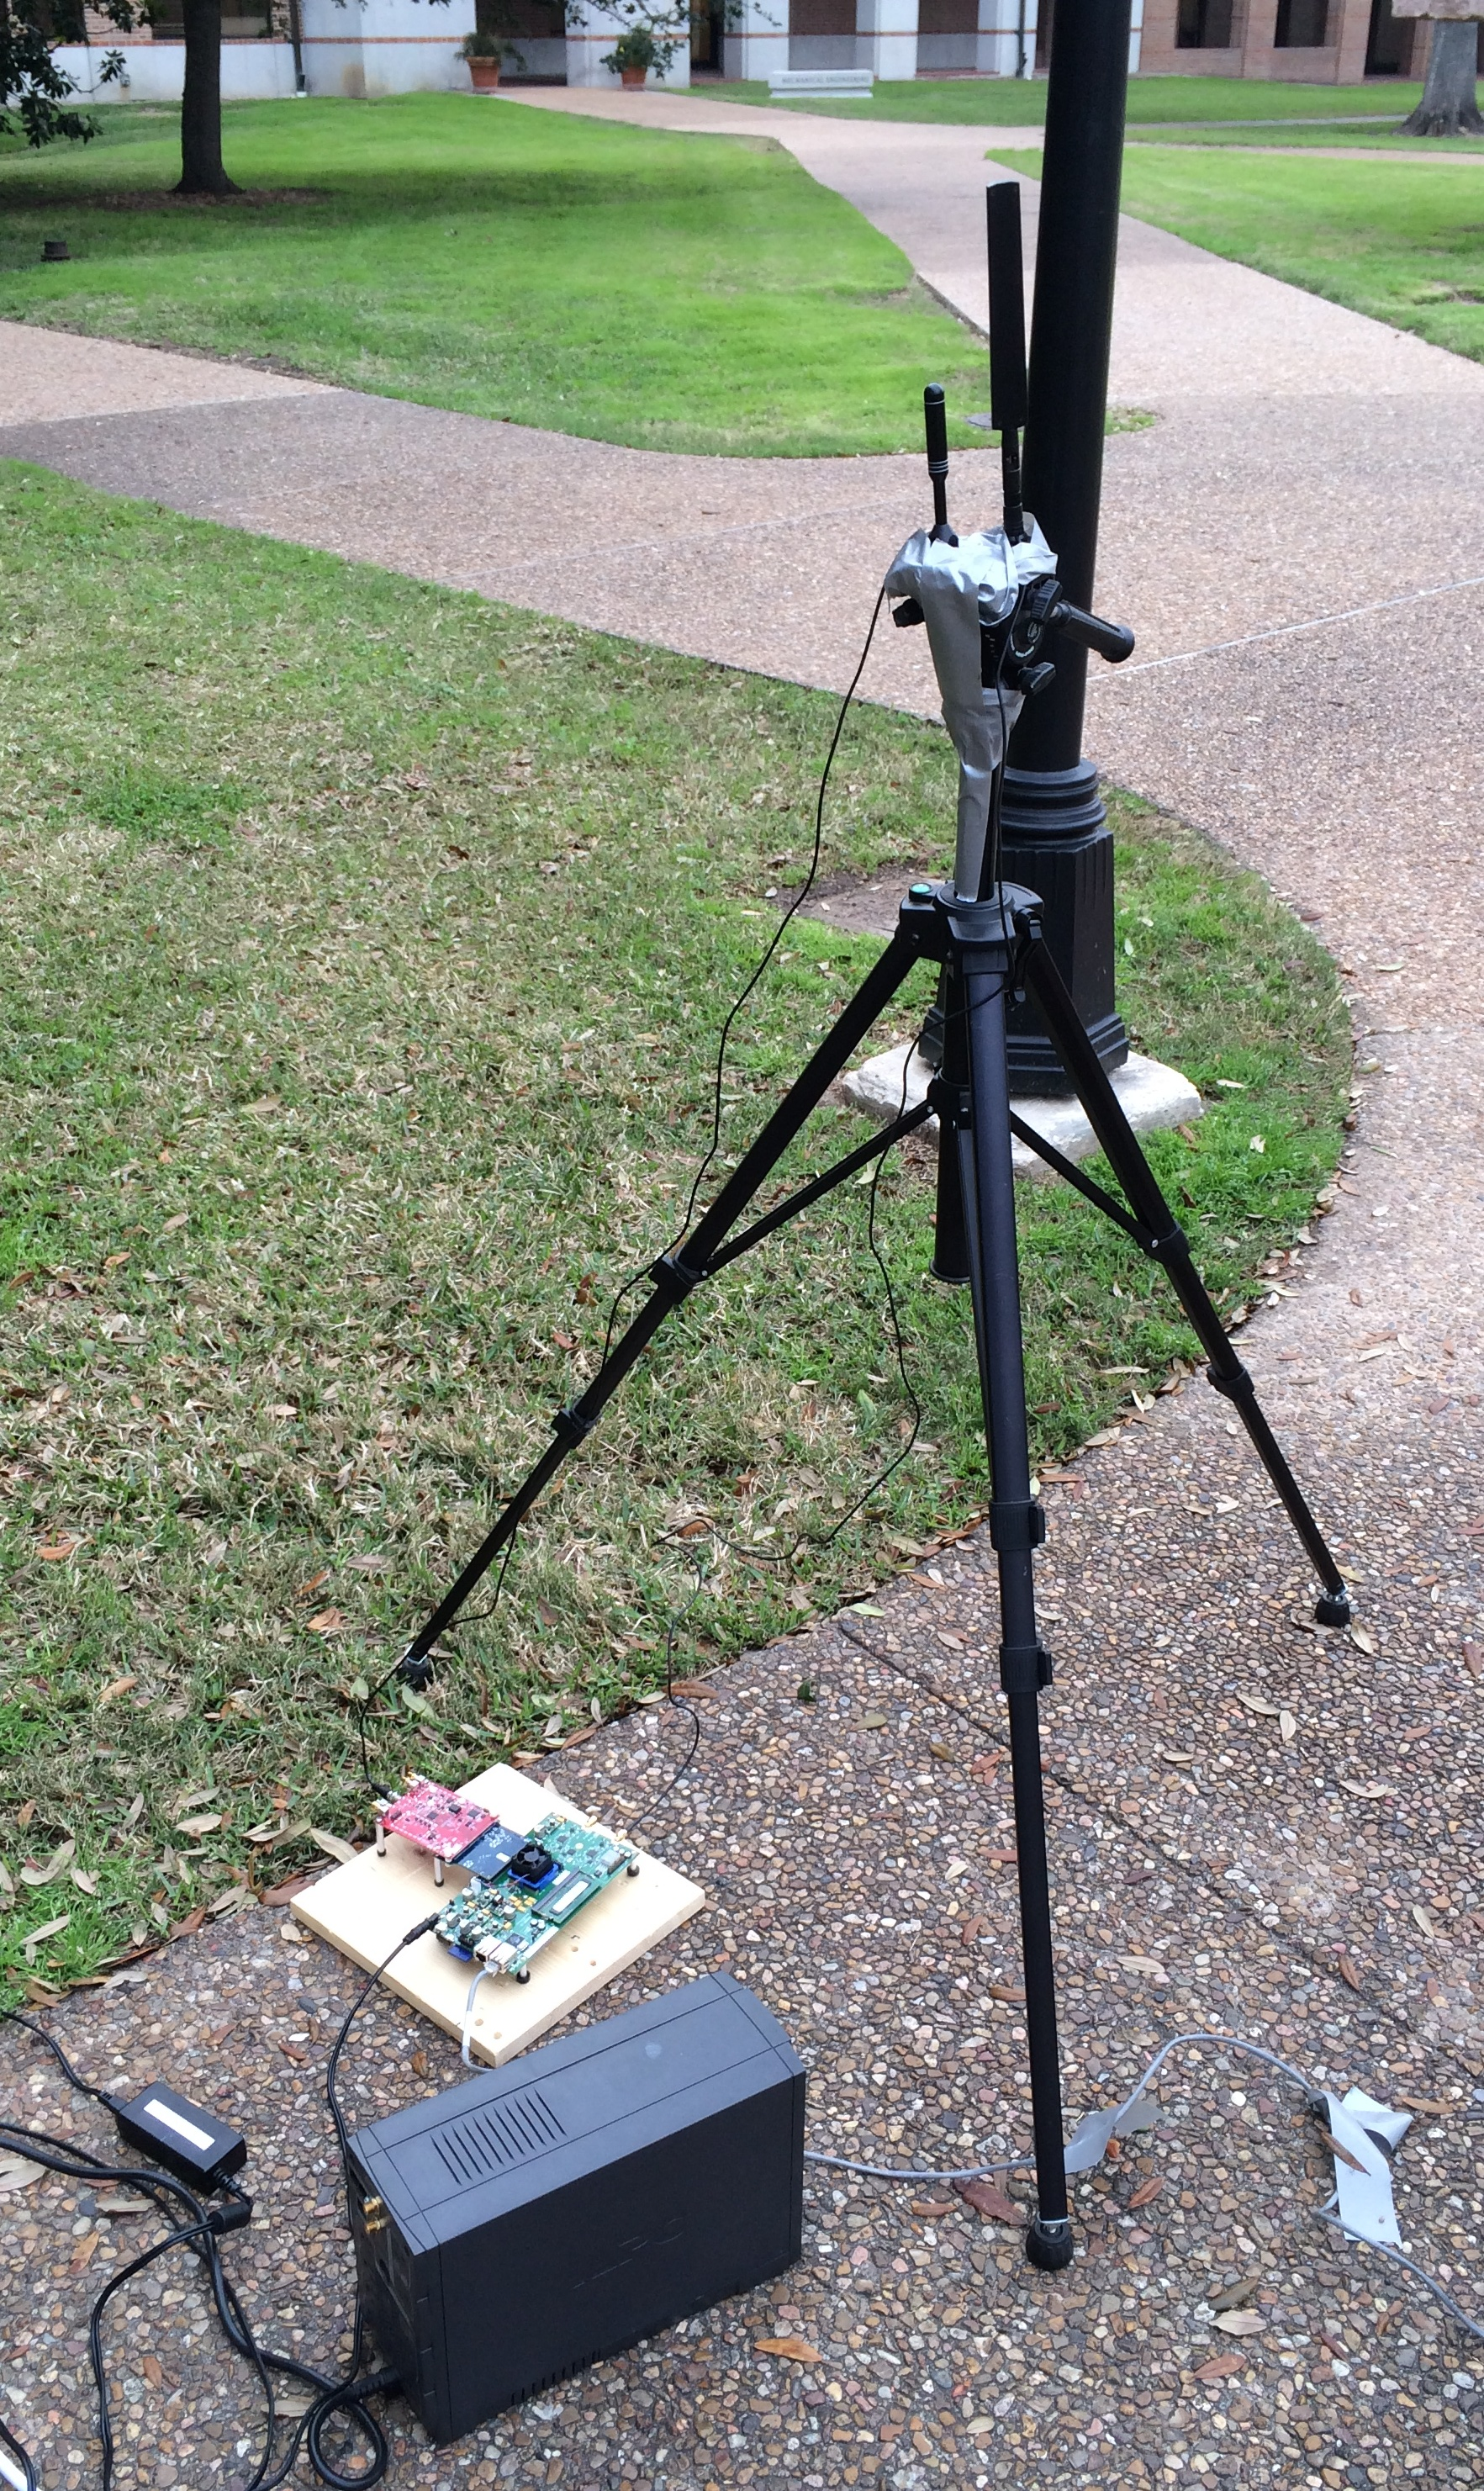
\includegraphics[width=0.48\linewidth]{figs/meas/ryan_tripod_platform}  
		\label{fig_fix_outdoor_sta}
	}
  	\caption{Fixed outdoor multi-band measurement setup \label{fig_fixed_outdoor}} 
\end{figure}

\section{Fixed Outdoor MU-MIMO Channel Characterization}

%\rgnote{TODO: I'm missing autocorrelation results from this experiment. Need to add.}

%\begin{figure}[th!]
%\centering
  %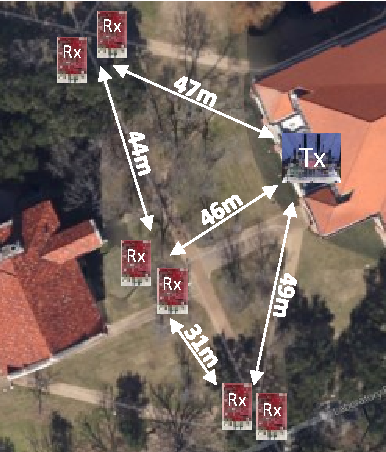
\includegraphics[width=0.5\linewidth]{figs/meas/outdoorExp}  
    %\caption{}\label{fig:outdoor}
%\end{figure}




	Finally, using the experimental framework developed in Section~\ref{sec_static_miso_chan_est}, we perform outdoor channel sounding experiments to directly compare the performance and stability of UHF \ac{MU-MIMO} channels.
	To that end, we setup an experimental network of a collection of nodes located outdoors being served by our array from a third floor balcony.  
	Although the UHF transmitter is capable of transmitting much further distances, we limited the scale of the topology as shown in Figure~\ref{fig_fix_outdoor_diagram} to ensure a fair comparison between UHF and 2.4/5~GHz bands.   
	The locations of the nodes were chosen such that the transmissions from the UHF and 2.4/5~GHz bands would reach the receivers (the UHF band transmitters can easily transmit further than 50~m).
	However, even by reducing the receiver distance to what is shown in Figure~\ref{fig_fix_outdoor_diagram}, the 5~GHz band transmissions did not reliably reach the receiving nodes.
	Since this severely limited the number of measured channel matrices at 5~GHz, we restrict our outdoor comparison to the UHF and 2.4~GHz bands.

	Just as we evaluated  temporal correlation in the multi-path rich, indoor transmission environment, we seek to similarly characterize the most detrimental aspect of the outdoor MU-MIMO channel: receiver separability.  
	Ill-conditioned channel matrices, as discussed in \S~\ref{sec:specDiff}, have a detrimental effect on an MU-MIMO enabled transmitter's ability to separate multiple users.  

	In the previous section, we found that while temporal stability of UHF was greater than that of 2.4/5 GHz, spatial correlation did not suffer as the UHF MU-MIMO transmissions were able to separate the co-located receivers.
	However, in an open, outdoor \ac{LoS} environment, we find that both the UHF and 2.4~GHz bands exhibit the same Demmel condition number. 
	Additionally, the CDF of the Demmel condition number closely matches the COST UHF channel condition shown in Fig.~\ref{fig:spatCorr}.
	This suggests that the comparison shown in Fig.~\ref{fig:spatCorr} is not a result of the frequency band itself, but rather the wholly different channel environments in which the model was parametrized.

\begin{figure}[t]
\centering
  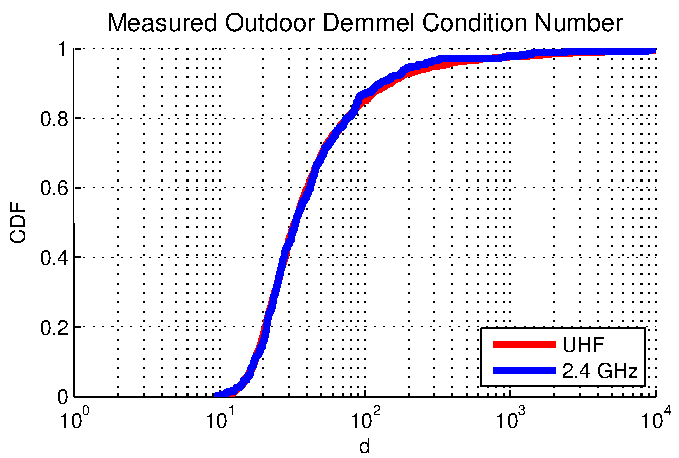
\includegraphics[width=0.7\linewidth]{figs/measSpatCorr}   
    \caption{Measured Demmel Condition Number of the outdoor MU-MIMO channel.}\label{fig:measSpat}
		\vspace{-5mm}
\end{figure}

%% UHF-band MUMIMO Conclusions
%\subsection{Discussion}
		%\rgnote{what does this mean for system design? the implications are very important}
